\section{Introduction to Organization}
Auribises offers a suite of mobile, web and software applications as a solution to industry.
\begin{figure}[ht]
\centering
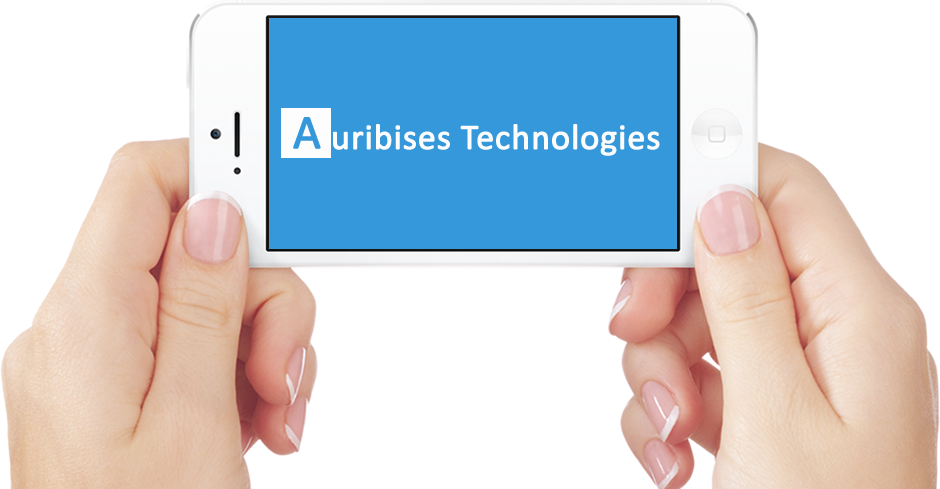
\includegraphics[scale=0.3]{images/aur.png}
\caption{Auribises}
\end{figure} 
We were founded in November 2011. With unparalleled domain competencies in mobile and web, Auribises is poised to take on critical challenges that the industry manifests. Our culture is values based, and we assure the highest ethical standards of integrity, transparency and corporate governance. Our value system is driven by STAR, the acronym for our core values of Share, Time, Achieve, and Respect. At Auribises, we just not only develop, but also provide educational services that helps students to hone their technical skills. Auribises offers a unique combination of technical competencies with practical exposure on ongoing projects to its students. Auribises has a core vision for lightening thousands of candles with a single candle and hence we believe that it is our endeavor to continually share our learning’s with the larger world.
\section{Introduction To Project} 
With the launch and increase in sales of smartphones over the last few years, people are using
mobile applications to get their work done, which makes their lives easier. Mobile applications
comprise various different categories such as Entertainment, Sports, Lifestyle, Education, Games,Food and Drink, Health and Fitness, Finance, etc. The application falls under Education category and helps the students as well as book nerds in sharing,storing and managing
their E-books.The software product went through the design, development, and the testing
phase as a part of the Software Development Lifecycle.

The applications interface is designed using custom art elements, the functionality is implemented using Android SDK, and the phase of testing the product was accomplished successfully. The application can very well manage,store and share different E-books among different users. User can upload and download E-books based upon preference.User can also enter
Description, date , name  and other optional attributes ( Adding categories  to the E-books). With this entered information, the user is able to see the name, file size, description, upload date and many other details of ebook. All these topics have been explained in detail in their respective chapters.

\section{Project Category}
This application is internet based android mobile application using real time NoSql database (Firebase Database).

\section{Objectives}

\begin{itemize}
	\item To make managing of ebooks easier.

	\item To easily find ebooks in various categories.
	
	\item To easily search through all the ebooks available.
	
	\item To easily share the ebook with anyone. 
\end{itemize}

\section{Problem Formulation}
An easy and stable platform for users who loves to read and share books. Helpful for the students, for managing their study material ex. ebook or pdf. They can easily access their material anytime and share it within groups or classmates. 

\section{Proposed System Modules}

\begin{itemize}
	\item Ebook Upload, Download, Delete, Share.

	\item Ebook arrange within category.
	
	\item Login Page(To ensure authenticated and secure system, system will have a login activity to ensure that only authorized user can use this system).
	
	\item Reset Password option.
\end{itemize}

 
\section{Unique Features of the System}
\begin{itemize}

\item Upload and Download Ebooks.
\item Arranging Ebooks in various categories.
\item User can delete the content uploaded by him/her.
\item Feedback option is given so that user can give opinion to admin.
\item User can search through all the the Ebooks available.
\item User can share the App as well as Ebook with anyone. 
\end{itemize}


